
\documentclass{article}

\title{A New Solution of Hydrogen}
\author{Brent Baccala}

\usepackage{amsmath}

\usepackage{xcolor}
\usepackage{comment}
\usepackage{graphicx}

\usepackage[hidelinks]{hyperref}

\usepackage{tabularx}

% For drawing ansatz diagrams

\usepackage{tikz}
\usetikzlibrary{calc}
\usetikzlibrary{positioning}
\usetikzlibrary{fit}
\usetikzlibrary{backgrounds}

\def\coeff{\framebox(10,10){}}
\newcommand{\tikzmark}[1]{\tikz[overlay,remember picture] \node (#1) {};}

\begin{document}
\parindent 0pt

\maketitle

\begin{abstract}
The author has developed a technique for finding exact solutions of partial
differential equations that does not require separation of variables
and is not a transform method.  As an illustration of the method,
I show a previously unknown exact solution to the simplest time-independent Schr\"odinger equation for hydrogen.
The solution involves a Bessel function, is not separable, and is not in $L^2$.
\end{abstract}

\subsection*{Introduction}
\parskip 12pt

The Schr\"odinger equation is the quantum mechanical equivalent of Newton's second law.
Both Newton's equation and Schr\"odinger's equation,
given a system of particles interacting under the influence of some force,
describe the time evolution of the system.  Newton's classical second law $F=ma$
describes the time evolution of the position and velocity of each particle.
Schr\"odinger's quantum mechanical formulation $H\Psi=i\frac{\delta}{\delta t} \Psi$
describes the time evolution
of the wavefunction $\Psi$, which is a complex-valued function of particle position
that encodes a probability density function for
the particle positions as $|\Psi|^2$ and a probability density function
for the particle momenta as $|\hat{\Psi}|^2$.

There is no one Schr\"odinger equation any more than there is one $F=ma$.
Each physical system under consideration gives rise to a different collection
of particles and interacting forces, and a different Hamiltonian operator $H$.
Indeed, even the approximations we
make strongly determine the form of the equation for a given system.

One of the simplest Schr\"odinger equations is for the hydrogen atom,
considering the electric force attraction between the nucleus and
the electronic, and ignoring all other effects.  It has the following form:

\begin{equation*}
%\label{schrodinger}
-\frac{1}{2}\nabla^2 \Psi - \frac{1}{r}\Psi = i \frac{\delta}{\delta t} \Psi
\end{equation*}

where $\Psi$ is the wavefunction, $\nabla^2$ is the Laplacian,
$r$ is the distance between the two particles, and $E$ is the
state's energy.

We can further simplify the general, time-dependent Schr\"odinger equation
by requiring that the position and momentum probability density functions
each be time-independent.  This restricts the solution to stable states
of the hydrogen atom, settles the wavefunction up to a multiple of $e^{itE}$,
and leads to the time-independent Schr\"odinger equation for hydrogen:

\begin{equation*}
%\label{schrodinger}
-\frac{1}{2}\nabla^2 \Psi - \frac{1}{r}\Psi = E \Psi
\end{equation*}

This equation is amenable to seperation of variables, leading to the
classical solutions, which have been known for a century:

TABLE

The classical solutions, in short, are separable, are in $L^2$, are in $C^\infty$,
and are each paired with a negative energy value, of which $-\frac{1}{2}$ is the lowest,
and corresponds to the 1s or ground state.

Yet the existance of separable solutions leaves open the existance of non-separable solutions.

The author has developed an algorithm to solve certain classes of ODEs

It is perhaps surprising that such a well-studied equation would have fairly simple, previously
undiscovered, non-separable solutions.

\subsection*{Theorem}
\parskip 0pt

Consider the following simple Sch\"odinger equation for the hydrogen atom:

\begin{equation}
\label{schrodinger}
-\frac{1}{2}\nabla^2 \Psi - \frac{1}{r}\Psi = E \Psi
\end{equation}

Let $J_0$ be the ordinary Bessel function $J_0$, and set

\begin{equation}
\label{solution}
\Psi = J_0(2\sqrt{x+r})
\end{equation}

where $x,y,z$ are Cartesian coordinates and $r=\sqrt{x^2+y^2+z^2}$.

\vskip 12pt

Then \eqref{solution} is an exact solution to \eqref{schrodinger}, with $E=0$.

\subsection*{Verification}

The result can be easily verified using Mathematica\footnote{A manual verification is presented in an appendix}, as follows:

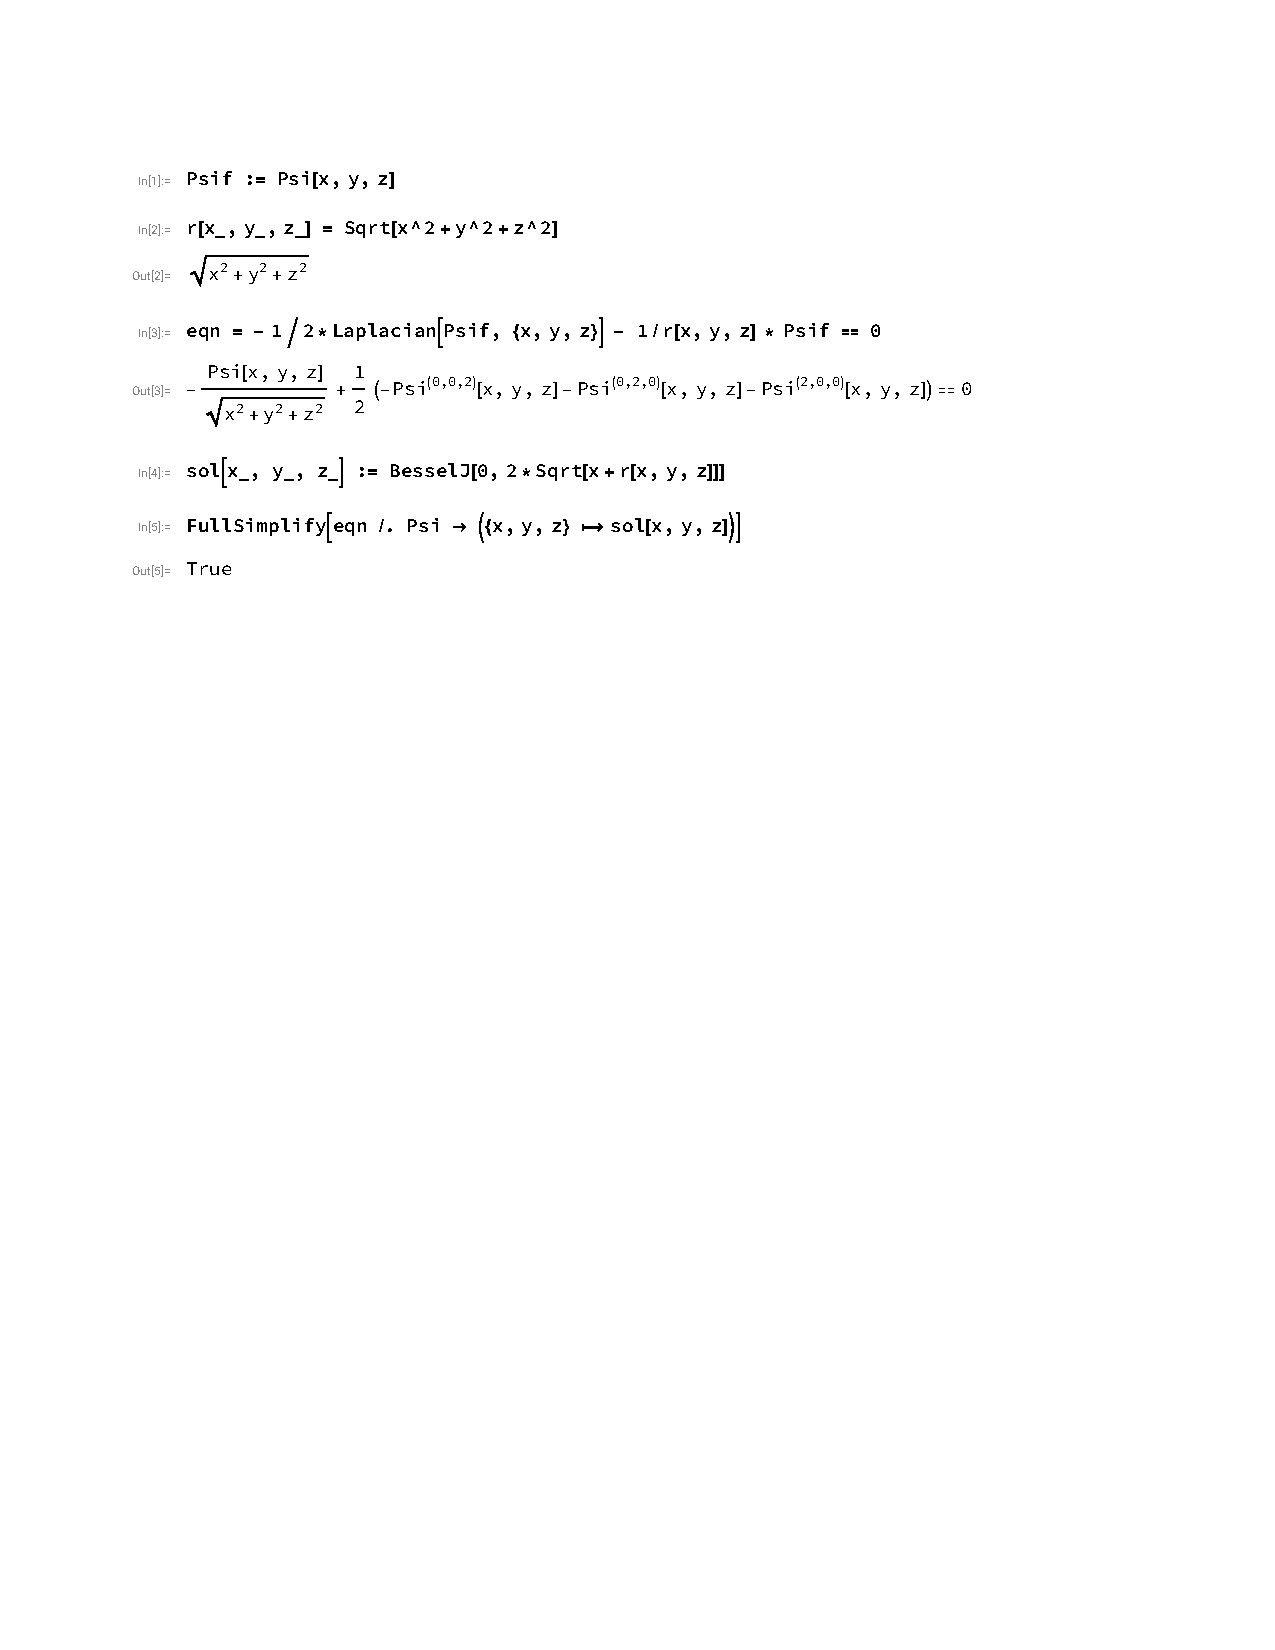
\includegraphics[page=1, clip, trim=1in 7in 1in 1in, width=\textwidth]{improved.pdf}

\subsection*{Generalization}
\parskip 12pt

The choice of $x$ is arbitrary, and any ordinary Bessel function can be used:

\begin{equation}
\label{generalized solution}
\Psi = F(2\sqrt{a_1 x+ a_2 y+ a_3 z+r})
\end{equation}

where

\begin{equation*}
a_1^2+a_2^2+a_3^2=1
\end{equation*}

and $F$ is any linear combination of the Bessel functions $J_0$ and $Y_0$.

\vskip 12pt

Any finite linear combination of functions of the form \eqref{generalized solution} also solves \eqref{schrodinger}.

\subsection*{Solution Method}

% I used a Sage-based computer program with the following ansatz.

I found this solution roughly as follows.\footnote{
I discovered an alternate form of this solution using a somewhat more complex ansatz
on January 24, 2023.  By January 26, I had established the solution in its current form.
The original ansatz produced a rational function with
a 1254 term numerator and a 36 term denominator, that gave rise to a system of 224 equations.
}

Use Cartesian coordinates.  Let $v$ be a linear polynomial in the coordinates and the root $r=\sqrt{x^2+y^2+z^2}$,
with the following form (the $v_i$ are constants):

\begin{equation}
\label{v ansatz}
v = v_0 r + v_1 x + v_2 y + v_3 z
\end{equation}

Assume the solution to the input PDE \eqref{schrodinger}
is a linear second-order ODE w.r.t. $v$ with linear coefficeints,
with the following form:

\begin{equation}
\label{psi ansatz}
(d_0 + d_1 v) \frac{\delta^2\Psi}{\delta v^2} - (m_0 + m_1 v) \frac{\delta\Psi}{\delta v} - (n_0 + n_1 v) \Psi = 0
\end{equation}

or:

\begin{equation}
\label{psi ansatz sub}
(d_0 + d_1 v) \frac{\delta^2\Psi}{\delta v^2} = (m_0 + m_1 v) \frac{\delta\Psi}{\delta v} + (n_0 + n_1 v) \Psi
\end{equation}

Substituting \eqref{v ansatz} into \eqref{psi ansatz sub}, expanding derivatives in \eqref{schrodinger},
substituting the RHS of \eqref{psi ansatz sub} into \eqref{schrodinger} where the LHS of
\eqref{psi ansatz sub} appears,
replacing all instances of $r^2$ with $x^2+y^2+z^2$, and canceling GCDs, we obtain a rational function
with a 228 term numerator and an 18 term denominator.  We ignore the denominator.  The numerator begins:

\begin{equation}
%% -8r\Psi x^5 b_1 b_2^2 n_1 - r\Psi x^5 b_1 b_4^2 n_1 - r \Psi x^5 b_1 b_6^2 n_1 - 2r\Psi x^5 b_2 b_3 b_4 n_1 - \cdots
-2r\Psi x^3 E d_1 v_1 - 3r\Psi x^3 n_1 v_0^2 v_1 - r\Psi x^3 n_1 v_1^3 - r\Psi x^3 n_1 v_1 v_2^2 - r\Psi x^3 n_1 v_1 v_3^2 - \cdots
\end{equation}

We collect like terms in $x$, $y$, $z$, $r$, $\Psi$, and $\Psi'$, organizing the numerator like this:

\begin{equation}
%%\left(-8 b_1 b_2^2 n_1 - b_1 b_4^2 n_1 - b_1 b_6^2 n_1 - 2 b_2 b_3 b_4 n_1 - 2b_2 b_5 b_6 n_1 \right) r\Psi x^5 - \cdots
r\Psi x^3 \left(-2 E d_1 v_1 - 3 n_1 v_0^2 v_1 - n_1 v_1^3 - n_1 v_1 v_2^2 - n_1 v_1 v_3^2\right) - \cdots
\end{equation}

The expressions in parenthesis gives us a system of equations (only one is shown)
involving the $v_i$, $d_i$, $m_i$ and $n_i$ variables that, if satisfied,
will yield a solution to \eqref{schrodinger} in the form \eqref{v ansatz} and \eqref{psi ansatz}.  Once
duplicate equations are dropped, the system has 34 equations.


%%sage: latex(matrix(eqns()).transpose())
\begin{equation}
\label{polynomial system}
\left(\begin{array}{r}
-2 \, n_{1} v_{0}^{3} - 4 \, n_{1} v_{0} v_{1}^{2} - 4 \, n_{1} v_{0} v_{2}^{2} - 2 \, n_{1} v_{0} v_{3}^{2} - 4 \, E d_{1} v_{0} \\
-2 \, n_{1} v_{0}^{3} - 4 \, n_{1} v_{0} v_{1}^{2} - 2 \, n_{1} v_{0} v_{2}^{2} - 4 \, n_{1} v_{0} v_{3}^{2} - 4 \, E d_{1} v_{0} \\
-2 \, n_{1} v_{0}^{3} - 2 \, n_{1} v_{0} v_{1}^{2} - 4 \, n_{1} v_{0} v_{2}^{2} - 4 \, n_{1} v_{0} v_{3}^{2} - 4 \, E d_{1} v_{0} \\
-4 \, m_{1} v_{0} v_{1} v_{2} \\
-4 \, m_{1} v_{0} v_{1} v_{3} \\
-4 \, m_{1} v_{0} v_{2} v_{3} \\
-4 \, n_{1} v_{0} v_{1} v_{2} \\
-4 \, n_{1} v_{0} v_{1} v_{3} \\
-4 \, n_{1} v_{0} v_{2} v_{3} \\
-3 \, m_{1} v_{0}^{2} v_{1} -  \, m_{1} v_{1}^{3} -  \, m_{1} v_{1} v_{2}^{2} -  \, m_{1} v_{1} v_{3}^{2} \\
-3 \, m_{1} v_{0}^{2} v_{2} -  \, m_{1} v_{1}^{2} v_{2} -  \, m_{1} v_{2}^{3} -  \, m_{1} v_{2} v_{3}^{2} \\
-3 \, m_{1} v_{0}^{2} v_{3} -  \, m_{1} v_{1}^{2} v_{3} -  \, m_{1} v_{2}^{2} v_{3} -  \, m_{1} v_{3}^{3} \\
-2 \, m_{1} v_{0}^{3} - 4 \, m_{1} v_{0} v_{1}^{2} - 4 \, m_{1} v_{0} v_{2}^{2} - 2 \, m_{1} v_{0} v_{3}^{2} \\
-2 \, m_{1} v_{0}^{3} - 4 \, m_{1} v_{0} v_{1}^{2} - 2 \, m_{1} v_{0} v_{2}^{2} - 4 \, m_{1} v_{0} v_{3}^{2} \\
-3 \, n_{1} v_{0}^{2} v_{1} -  \, n_{1} v_{1}^{3} -  \, n_{1} v_{1} v_{2}^{2} -  \, n_{1} v_{1} v_{3}^{2} - 2 \, E d_{1} v_{1} \\
-3 \, n_{1} v_{0}^{2} v_{2} -  \, n_{1} v_{1}^{2} v_{2} -  \, n_{1} v_{2}^{3} -  \, n_{1} v_{2} v_{3}^{2} - 2 \, E d_{1} v_{2} \\
-3 \, n_{1} v_{0}^{2} v_{3} -  \, n_{1} v_{1}^{2} v_{3} -  \, n_{1} v_{2}^{2} v_{3} -  \, n_{1} v_{3}^{3} - 2 \, E d_{1} v_{3} \\
-2 \, m_{1} v_{0}^{3} - 2 \, m_{1} v_{0} v_{1}^{2} - 4 \, m_{1} v_{0} v_{2}^{2} - 4 \, m_{1} v_{0} v_{3}^{2} \\
- \, n_{0} v_{0}^{2} -  \, n_{0} v_{1}^{2} -  \, n_{0} v_{2}^{2} -  \, n_{0} v_{3}^{2} - 2 \, E d_{0} - 2 \, d_{1} v_{0} \\
-2 \, n_{0} v_{0} v_{1} - 2 \, d_{1} v_{1} \\
-2 \, n_{0} v_{0} v_{2} - 2 \, d_{1} v_{2} \\
-2 \, n_{0} v_{0} v_{3} - 2 \, d_{1} v_{3} \\
-2 \, d_{1} v_{0} v_{1} - 2 \, m_{0} v_{0} v_{1} \\
-2 \, d_{1} v_{0} v_{2} - 2 \, m_{0} v_{0} v_{2} \\
-2 \, d_{1} v_{0} v_{3} - 2 \, m_{0} v_{0} v_{3} \\
- \, n_{1} v_{0}^{3} - 3 \, n_{1} v_{0} v_{1}^{2} -  \, n_{1} v_{0} v_{2}^{2} -  \, n_{1} v_{0} v_{3}^{2} - 2 \, E d_{1} v_{0} \\
- \, n_{1} v_{0}^{3} -  \, n_{1} v_{0} v_{1}^{2} - 3 \, n_{1} v_{0} v_{2}^{2} -  \, n_{1} v_{0} v_{3}^{2} - 2 \, E d_{1} v_{0} \\
- \, n_{1} v_{0}^{3} -  \, n_{1} v_{0} v_{1}^{2} -  \, n_{1} v_{0} v_{2}^{2} - 3 \, n_{1} v_{0} v_{3}^{2} - 2 \, E d_{1} v_{0} \\
-2 \, d_{1} v_{0}^{2} -  \, m_{0} v_{0}^{2} -  \, m_{0} v_{1}^{2} -  \, m_{0} v_{2}^{2} -  \, m_{0} v_{3}^{2} \\
-2 \, d_{0} \\
-2 \, d_{0} v_{0} \\
- \, m_{1} v_{0}^{3} - 3 \, m_{1} v_{0} v_{1}^{2} -  \, m_{1} v_{0} v_{2}^{2} -  \, m_{1} v_{0} v_{3}^{2} \\
- \, m_{1} v_{0}^{3} -  \, m_{1} v_{0} v_{1}^{2} - 3 \, m_{1} v_{0} v_{2}^{2} -  \, m_{1} v_{0} v_{3}^{2} \\
- \, m_{1} v_{0}^{3} -  \, m_{1} v_{0} v_{1}^{2} -  \, m_{1} v_{0} v_{2}^{2} - 3 \, m_{1} v_{0} v_{3}^{2}
\end{array}\right)
\end{equation}

Several solution techniques are available to solve a system of polynomial equations; I used
a numerical approximation technique.  A laptop computer finds the following approximate solution
in less than three seconds:

\begin{equation}
\label{witness point}
\addtolength{\jot}{-3pt}
\begin{aligned}
&\verb!(E, 1.2793593235207163e-32)!\\
&\verb!(d0, 1.4231937528298923e-43)!\\
&\verb!(d1, 1.0)!\\
&\verb!(m0, -1.0)!\\
&\verb!(m1, 5.0839108285704363e-42)!\\
&\verb!(n0, -1.0)!\\
&\verb!(n1, -8.795561312674161e-33)!\\
&\verb!(v0, 1.0)!\\
&\verb!(v1, 0.47255672374941904)!\\
&\verb!(v2, 0.5379975369878418)!\\
&\verb!(v3, 0.6980320859632679)!
\end{aligned}
\end{equation}

This is a {\it witness point},\footnote{a term common in the literature} an approximate solution accurate enough
to recover an exact solution.

In this case, exactness recovery is simple and straightforward.  $E$, $d_0$, $m_1$ and $n_1$ are all quite small,
so we set them to zero, while $d_1$, $m_0$, $n_0$ and $v_0$ already have their exact values and:

\begin{equation*}
0.4725567237^2 + 0.5379975369^2 + 0.6980320859^2 \approx  1.0000000000
\end{equation*}

so we add $v_1^2 + v_2^2 + v_3^2 = 1$ to our solution and conclude that our witness point lies approximately
on the following algebraic variety:

\begin{equation}
\begin{gathered}
E = 0 \\
d_0 = 0 \qquad
d_1 = 1 \\
m_0 = -1 \qquad
m_1 = 0 \\
n_0 = -1 \qquad
n_1 = 0 \\
v_0 = 1 \qquad
v_1^2 + v_2^2 + v_3^2 = 1
\end{gathered}
\end{equation}

Substituting these values back into our ansatz, we conclude that $\Psi(v)$
is a solution of \eqref{schrodinger} under these conditions:

\begin{equation}
\label{related solution}
\begin{gathered}
v \frac{\delta^2\Psi}{\delta v^2} + \frac{\delta\Psi}{\delta v} + \Psi = 0 \\
v = v_1 x+ v_2 y+ v_3 z+r \\
v_1^2 + v_2^2 + v_3^2 = 1
\end{gathered}
\end{equation}

We now have to solve a second order ODE:

\begin{equation}
v \Psi''(v) + \Psi'(v) + \Psi(v) = 0
\end{equation}

Wolfram Mathematica\footnote{I originally used Wolfram Alpha} can now
analyze this equation and determine that it is equivalent
to the Bessel function \eqref{solution}.

\includegraphics[page=1, clip, trim=1in 9in 1in 1in, width=\textwidth]{find Bessel solution.pdf}

\subsection*{Software}

The program used to find the witness point is available here:

\centerline{\url{https://github.com/BrentBaccala/helium}}

It's a Sage script that works fine with Sage 9.0 on Ubuntu 20.

Use it to find the witness point \eqref{witness point} by
running Sage as follows:

\begin{verbatim}
load('helium.sage')     # loads the script
prep_hydrogen(5)        # select PDE:hydrogen and ansatz:5
multi_init()            # form the equation
multi_expand()          # expand out the numerator and collect like terms into a matrix
random_numerical()      # run numerical optimizer
\end{verbatim}

Here are some other convenient variables and functions in the script:

\begin{verbatim}
V, D, N, M              # trial forms of various polynomials
eq_a                    # PDE with ansatz substituted in and r^2 simplified
R                       # polynomial ring over integers
F                       # fraction field of R
F_eq_a                  # eq_a expanded out (in F)
F_eq_a_n                # expanded numerator (in R)
F_eq_a_d                # expanded denominator (in R)
eqns()                  # system of equations to solve
SciMin                  # solution from scipy.optimize.root
\end{verbatim}

\subsection*{Exact Methods}

I used a numerical algorithm to solve the system of equations in expectation
of it being faster for larger systems, but the system \eqref{polynomial system}
is small enough that exact methods are usable.  In particular, we can form
an ideal $I$ in $\mathbf{Q}[v_0,...,m_1,E]$ from \eqref{polynomial system}.
Sage can calculate a Gr\"obner basis for the radical $I$ in less than a second.
While we could work with the Gr\"obner basis directly\footnote{A Gr\"obner basis
of the solution ideal in lexicographic order $E>d_i>m_i>n_i>v_i$ contains 65 polynomials.}
, I find it more
useful to study the primary decomposition, which Sage computes using
the Shimoyama-Yokoyama algorithm\footnote{Localization and Primary Decomposition of
Polynomial Ideals, {\it J. Symbolic Computation} (1996) {\bf 22}, 247–277}
as implemented in Singular.  Gr\"obner basis calculations are done
as a subalgorithm of Shimoyama-Yokoyama.

\begin{subequations}
%% sage: list(map(latex, I.radical().primary_decomposition()))
%% \Bold.* -> \\
\begin{align}
& \left(v_{0}^{2} - v_{1}^{2} - v_{2}^{2} - v_{3}^{2}, n_{1}, m_{1}, m_{0} - n_{0} v_{0}, d_{1} + n_{0} v_{0}, d_{0}, E\right)\label{ideal:1} \\
& \left(v_{3}, v_{2}, v_{1}, m_{1}, m_{0} - n_{0} v_{0}, 2 d_{1} + n_{0} v_{0}, d_{0}, E n_{0} - n_{1} v_{0}\right)\label{ideal:2}\\
& \left(v_{1}^{2} + v_{2}^{2} + v_{3}^{2}, v_{0}, d_{1}, d_{0}\right)\label{ideal:3}\\
& \left(v_{3}, v_{2}, v_{1}, v_{0}, d_{0}\right)\label{ideal:4}\\
& \left(n_{1}, n_{0}, m_{1}, m_{0}, d_{1}, d_{0}\right)\label{ideal:5}
\end{align}
\end{subequations}

Several of these varieties solve the system of equations, but do not lead to a meaningful solution to the differential equation.
In brief,

\begin{itemize}
\item[\eqref{ideal:1}] corresponds to our new solution (see below),
\item[\eqref{ideal:2}] corresponds to the classical solutions (see below),
\item[\eqref{ideal:3}] sets the coefficient of
%$\frac{d^2\Psi}{dv^2}$
$D^2\Psi$
in the ODE to zero, resulting in a first-order ODE, so we discard it,
\item[\eqref{ideal:4}] sets the variable $v$ to zero, so we discard it,
\item[\eqref{ideal:5}] sets all coefficients of the ODE to zero, so we discard it, too.

\end{itemize}

How to understand ideal \eqref{ideal:2}?  $d_0$ is an ideal generator,
so $d_0=0$, and we can always multiply our DE by a constant without affecting our result, so we can set $d_1=1$.
Likewise, we can multiply our variable $v$ by a constant and that will only change our coefficients by constants,
and $v_1=v_2=v_3=0$, so we can normalize by setting $v_0=1$.  This simplifies ideal \eqref{ideal:2} to:

\begin{equation}
\left(v_{3}, v_{2}, v_{1}, v_{0} - 1, n_{0} + 2, m_{1}, m_{0} + 2, d_{1} - 1, d_{0}, 2 E + n_{1}\right)
\end{equation}

\begin{equation}
\label{classical eq in ideal}
\begin{gathered}
v=r \\
v \Psi'' + 2 \Psi' + 2(1 + E v) \Psi = 0
\end{gathered}
\end{equation}

This is the classical radial equation obtained by seperation of variables\footnote{See
Pauling and Wilson or
\url{http://hyperphysics.phy-astr.gsu.edu/hbase/quantum/hydrad.html}}.  We use
spherical coordinates, set $\Psi = R(r)P(\theta)F(\psi)$, and obtain the above equation for $R(r)$,
though it is more commonly written in this form:

\begin{equation}
\frac{1}{R} \frac{d}{dr}\left[ r^2 \frac{dR}{dr}\right] + 2(Er^2 + r) = l(l+1)
\end{equation}

where $l$ is the orbital quantum number, which can be zero.  Set $l=0$, $v=r$ and $\Psi=R$ and
expand out the derivative to obtain \eqref{classical eq in ideal}.  Its presence here was
expected and won't be commented on further.

Ideal \eqref{ideal:1} was not expected, and contains our new solution.  Does it contain any additional solutions?
$d_0$ is an ideal generator,
so $d_0=0$, and we can set $d_1=1$, by the same logic as above.
Our coordinates are in real space, so our $v_i$ coefficients must be real (why?), so all of their squares must
be positive, and since $v_0^2-v_1^2-v_2^2-v_3^3=0$, $v_0$ must be non-zero.  So we can normalize by setting $v_0=1$.
That simplifies \eqref{ideal:1} to this:

\begin{equation}
\left(v_{1}^{2} + v_{2}^{2} + v_{3}^{2} - 1, v_{0} - 1, n_{1}, n_{0} + 1, m_{1}, m_{0} + 1, d_{1} - 1, d_{0}, E\right)
\end{equation}

So we conclude that \eqref{ideal:1} contains only our new solution and simple variants thereof.

\subsection*{The Rosenfeld-Gr\"obner algorithm}

\subsection*{The Ansatzen}

These are current and future ansatzen for the form of the ODE:

For hydrogen, the PDE is always $\nabla^2 \Psi - \frac{1}{r} \Psi = E \Psi$

\begin{itemize}
\item[Ansatz 1:] Exponential of a first degree polynomial times a first degree polynomial

Expected to find 1s and 2s levels of hydrogen, $e^{-r}$ and $(2-r)e^{r/2}$

$A,B \in \mathbf{C}[x,y,z,r]; \deg A \le 1; \deg B \le 1$

$\Psi = A F; F' = F; F_x = B_x F'; F_y = B_y F'; F_z = B_z F'$

or just: $\Psi = A F; F_x = B_x F; F_y = B_y F; F_z = B_z F$

Example: $B=-r; A=1; E=-1/2$ $\qquad\Rightarrow\qquad$ $e^{-r}$

Example: $B=-r/2; A=r-2; E=-1/8$ $\qquad\Rightarrow\qquad$ $(2-r)e^{-r/2}$

\item[Ansatz 2:] Logarithm of a first degree polynomial times a first degree polynomial

$A,B \in \mathbf{C}[x,y,z,r]; \deg A \le 1; \deg B \le 1$

$\Psi = A F; F' = 1/F; F_x = B_x F'; F_y = B_y F'; F_z = B_z F'$

or just: $\Psi = A F; F_x = B_x / F; F_y = B_y / F; F_z = B_z / F$

\item[Ansatz 3,4:] Unused

\item[Ansatz 5:] Second-order ODE with linear coefficients and a linear variable

Expected to find 1s level of hydrogen, $e^{-r}$

$A,B,C,V \in \mathbf{C}[x,y,z,r]; \deg A \le 1; \deg B \le 1; \deg C \le 1; \deg V \le 1$

$\Psi = F; A F'' + B F' + C F = 0; F_x = V_x F'; F_y = V_y F'; F_z = V_z F'$

Example: $V=-r; A+C=-B; E=-1/2$ ($A, B, C \in \mathbf{C}$) $\Rightarrow$ $e^{-r}$

\item[Ansatz 6:] Second-order ODE with linear coefficients and a first-degree rational function variable

\item[Ansatz 7:] Second-order ODE with second-degree coefficients and a second-degree rational function variable

\item[Ansatz 8:] (logically before ansatz 5) First-order ODE with linear coefficients and a linear polynomial variable

\item[Ansatz 9:] (logically before ansatz 8) First-order ODE with constant coefficients and a linear polynomial variable

\item[Ansatz 10:] (logically before ansatz 7) Second-order ODE with second-degree coefficients and a second-degree polynomial variable

\item[Ansatz 11:] An second-degree algebraic extension with second-degree coefficients (involving $E$?),
followed by ansatz 7 (second-order ODE with second-degree coefficients and a second-degree rational function variable)

\item[Ansatz 12:] Two nested second-order ODEs with second-degree coefficients and a second-degree rational function variable (ansatz 7 twice)

\item[Ansatz 13:] Ansatz 11 twice

\end{itemize}

\subsection*{The Algorithm}

Given a PDE defined by Ritt-type differential polynomials, attempt the following:

1. Select an ansatz that defines a differential space parameterized by constants (see next section)

2. Reduce the PDE modulo the differential ideal that characterizes the differential space (differential elimination step)

3. Construct a system of polynomial equations in the constants by collecting like terms in the remaining variables

4. Construct the ideal I defined by that system of polynomial equations as generators

5. Are there any zero divisors in the differential space? (probably not)  If not, take the radical of I.

6. Construct the primary decomposition (prime decomposition if I is radical)

7. Each ideal in the primary/prime decomposition corresponds to a variety in the space of constants,
the union of which form the solution space of the PDE in the differential space.

\subsection*{Ansatz Diagrams}

The algorithm requires selection of an {\bf ansatz}, which is a differential
algebraic function space, based on the coefficient ring used to define the PDE,
and built using a finite sequence of ODE and algebraic extensions.  An
ansatz is also required to be parametized by a finite number of constants,
so degree bounds, for example, are required for most polynomials.

I've developed a graphical notation to describe an ansatz.  Blue-purple boxes
denote rings, orange boxes (whether shaded orange or not) denote ODE extensions, and green boxes denote
algebraic extensions.  A blue box drawn immediately around an orange or green box
denote the ring formed by adjoining the element defined by the orange or green box.
Polynomials are drawn as a square white box and are
connected by a line to the ring to which they belong.  A number next to
the line indicates a degree bound on the polynomial, and two numbers
separated by a slash denote a rational function.  For example, 2/2 denotes
a rational function with a second degree numerator and a second degree
denominator.

\tikzstyle{poly}=[rectangle, draw, thick, fill=white, text width=5em, align=center, rounded corners, minimum height=2em]
\tikzstyle{ring}=[rectangle, draw=blue, thick, fill=blue!20, text width=5em,align=center, rounded corners, minimum height=2em]
\tikzstyle{element}=[rectangle, draw=orange, thick, fill=orange!20, align=center, rounded corners, minimum height=2em]
\tikzstyle{algebraic}=[rectangle, draw=green, thick, fill=green!20, align=center, rounded corners, minimum height=2em]
\tikzstyle{degree}=[]

{\bf Ansatz 9}

  \begin{tikzpicture}[remember picture,out=315,in=225,distance=0.4cm,node distance=40pt]
    \node (Psi) [poly, text width=100pt] {$\framebox(10,10){}\tikzmark{a}\,\Psi' + \coeff\tikzmark{b}\,\Psi$};
    \node (Qv) [ring, below of=Psi, text width=100pt] {$\mathbf{Q}[v]$};
    \node (v) [poly, right=of Qv] {$v$};
    \draw[degree] (a.west) -- (a.west|-Qv.north) node[right,pos=0.6] {0};
    \draw[degree] (b.west) -- (b.west|-Qv.north) node[right,pos=0.6] {0};
    \node (Psi label) [at=(v.east|-Psi.north), anchor=north east] {\Large$\Psi$};
    \begin{scope}[on background layer]
        \node (Psi block)[fit=(Psi) (Qv) (v), inner sep=10pt, element] {};
    \end{scope}
    \node (base) [ring, node distance=70pt, below=of Psi block.east, anchor=east, text width=250pt] {$\mathbf{Q}[x,y,z,r]/(r^2-x^2-y^2-z^2)$};
    \draw[degree] (v.south) -- (v.south|-base.north) node[right,pos=0.7] {1};
  \end{tikzpicture}

{\bf Ansatz 8}

  \begin{tikzpicture}[remember picture,out=315,in=225,distance=0.4cm,node distance=40pt]
    \node (Psi) [poly, text width=100pt] {$\framebox(10,10){}\tikzmark{a}\,\Psi' + \coeff\tikzmark{b}\,\Psi$};
    \node (Qv) [ring, below of=Psi, text width=100pt] {$\mathbf{Q}[v]$};
    \node (v) [poly, right=of Qv] {$v$};
    \draw[degree] (a.west) -- (a.west|-Qv.north) node[right,pos=0.6] {1};
    \draw[degree] (b.west) -- (b.west|-Qv.north) node[right,pos=0.6] {1};
    \node (Psi label) [at=(v.east|-Psi.north), anchor=north east] {\Large$\Psi$};
    \begin{scope}[on background layer]
        \node (Psi block)[fit=(Psi) (Qv) (v), inner sep=10pt, element] {};
    \end{scope}
    \node (base) [ring, node distance=70pt, below=of Psi block.east, anchor=east, text width=250pt] {$\mathbf{Q}[x,y,z,r]/(r^2-x^2-y^2-z^2)$};
    \draw[degree] (v.south) -- (v.south|-base.north) node[right,pos=0.7] {1};
  \end{tikzpicture}

{\bf Ansatz 5}

  \begin{tikzpicture}[remember picture,out=315,in=225,distance=0.4cm,node distance=40pt]
    \node (Psi) [poly, text width=100pt] {$\framebox(10,10){}\tikzmark{a}\,\Psi'' + \framebox(10,10){}\tikzmark{b}\,\Psi' + \coeff\tikzmark{c}\,\Psi$};
    \node (Qv) [ring, below of=Psi, text width=100pt] {$\mathbf{Q}[v]$};
    \node (v) [poly, right=of Qv] {$v$};
    \draw[degree] (a.west) -- (a.west|-Qv.north) node[right,pos=0.6] {1};
    \draw[degree] (b.west) -- (b.west|-Qv.north) node[right,pos=0.6] {1};
    \draw[degree] (c.west) -- (c.west|-Qv.north) node[right,pos=0.6] {1};
    \node (Psi label) [at=(v.east|-Psi.north), anchor=north east] {\Large$\Psi$};
    \begin{scope}[on background layer]
        \node (Psi block)[fit=(Psi) (Qv) (v), inner sep=10pt, element] {};
    \end{scope}
    \node (base) [ring, node distance=70pt, below=of Psi block.east, anchor=east, text width=250pt] {$\mathbf{Q}[x,y,z,r]/(r^2-x^2-y^2-z^2)$};
    \draw[degree] (v.south) -- (v.south|-base.north) node[right,pos=0.7] {1};
  \end{tikzpicture}

\vbox{
{\bf Ansatz 6}

  \begin{tikzpicture}[remember picture,out=315,in=225,distance=0.4cm,node distance=40pt]
    \node (Psi) [poly, text width=100pt] {$\framebox(10,10){}\tikzmark{a}\,\Psi'' + \framebox(10,10){}\tikzmark{b}\,\Psi' + \coeff\tikzmark{c}\,\Psi$};
    \node (Qv) [ring, below of=Psi, text width=100pt] {$\mathbf{Q}[v]$};
    \node (v) [poly, right=of Qv] {$v$};
    \draw[degree] (a.west) -- (a.west|-Qv.north) node[right,pos=0.6] {1};
    \draw[degree] (b.west) -- (b.west|-Qv.north) node[right,pos=0.6] {1};
    \draw[degree] (c.west) -- (c.west|-Qv.north) node[right,pos=0.6] {1};
    \node (Psi label) [at=(v.east|-Psi.north), anchor=north east] {\Large$\Psi$};
    \begin{scope}[on background layer]
        \node (Psi block)[fit=(Psi) (Qv) (v), inner sep=10pt, element] {};
    \end{scope}
    \node (base) [ring, node distance=70pt, below=of Psi block.east, anchor=east, text width=250pt] {$\mathbf{Q}[x,y,z,r]/(r^2-x^2-y^2-z^2)$};
    \draw[degree] (v.south) -- (v.south|-base.north) node[right,pos=0.7] {1/1};
  \end{tikzpicture}
}

{\bf Ansatz 7}

  \begin{tikzpicture}[remember picture,out=315,in=225,distance=0.4cm,node distance=40pt]
    \node (Psi) [poly, text width=100pt] {$\framebox(10,10){}\tikzmark{a}\,\Psi'' + \framebox(10,10){}\tikzmark{b}\,\Psi' + \coeff\tikzmark{c}\,\Psi$};
    \node (Qv) [ring, below of=Psi, text width=100pt] {$\mathbf{Q}[v]$};
    \node (v) [poly, right=of Qv] {$v$};
    \draw[degree] (a.west) -- (a.west|-Qv.north) node[right,pos=0.6] {2};
    \draw[degree] (b.west) -- (b.west|-Qv.north) node[right,pos=0.6] {2};
    \draw[degree] (c.west) -- (c.west|-Qv.north) node[right,pos=0.6] {2};
    \node (Psi label) [at=(v.east|-Psi.north), anchor=north east] {\Large$\Psi$};
    \begin{scope}[on background layer]
        \node (Psi block)[fit=(Psi) (Qv) (v), inner sep=10pt, element] {};
    \end{scope}
    \node (base) [ring, node distance=70pt, below=of Psi block.east, anchor=east, text width=250pt] {$\mathbf{Q}[x,y,z,r]/(r^2-x^2-y^2-z^2)$};
    \draw[degree] (v.south) -- (v.south|-base.north) node[right,pos=0.7] {2/2};
  \end{tikzpicture}

{\bf Ansatz 10}

  \begin{tikzpicture}[remember picture,out=315,in=225,distance=0.4cm,node distance=40pt]
    \node (Psi) [poly, text width=100pt] {$\framebox(10,10){}\tikzmark{a}\,\Psi'' + \framebox(10,10){}\tikzmark{b}\,\Psi' + \coeff\tikzmark{c}\,\Psi$};
    \node (Qv) [ring, below of=Psi, text width=100pt] {$\mathbf{Q}[v]$};
    \node (v) [poly, right=of Qv] {$v$};
    \draw[degree] (a.west) -- (a.west|-Qv.north) node[right,pos=0.6] {2};
    \draw[degree] (b.west) -- (b.west|-Qv.north) node[right,pos=0.6] {2};
    \draw[degree] (c.west) -- (c.west|-Qv.north) node[right,pos=0.6] {2};
    \node (Psi label) [at=(v.east|-Psi.north), anchor=north east] {\Large$\Psi$};
    \begin{scope}[on background layer]
        \node (Psi block)[fit=(Psi) (Qv) (v), inner sep=10pt, element] {};
    \end{scope}
    \node (base) [ring, node distance=70pt, below=of Psi block.east, anchor=east, text width=250pt] {$\mathbf{Q}[x,y,z,r]/(r^2-x^2-y^2-z^2)$};
    \draw[degree] (v.south) -- (v.south|-base.north) node[right,pos=0.7] {2};
  \end{tikzpicture}


\vbox{
{\bf Ansatz 11}

  \begin{tikzpicture}[remember picture,out=315,in=225,distance=0.4cm,node distance=40pt]
    \node (Psi) [poly, text width=100pt] {$\framebox(10,10){}\tikzmark{a}\,\Psi'' + \framebox(10,10){}\tikzmark{b}\,\Psi' + \coeff\tikzmark{c}\,\Psi$};
    \node (Qv) [ring, below of=Psi, text width=100pt] {$\mathbf{Q}[v]$};
    \node (v) [poly, right=of Qv] {$v$};
    \draw[degree] (a.west) -- (a.west|-Qv.north) node[right,pos=0.6] {2};
    \draw[degree] (b.west) -- (b.west|-Qv.north) node[right,pos=0.6] {2};
    \draw[degree] (c.west) -- (c.west|-Qv.north) node[right,pos=0.6] {2};
    \node (Psi label) [at=(v.east|-Psi.north), anchor=north east] {\Large$\Psi$};
    \begin{scope}[on background layer]
        \node (Psi block)[fit=(Psi) (Qv) (v), inner sep=10pt, element] {};
    \end{scope}
    \node (alg ext) [poly, node distance=150pt, below=of Psi.east, anchor=east, text width=100pt] {$\framebox(10,10){}\tikzmark{a}\,\gamma^2 + \framebox(10,10){}\tikzmark{b}\,\gamma + \coeff\tikzmark{c}$};
    \begin{scope}[on background layer]
        \node (alg ext element) [algebraic, fit=(alg ext) (Psi label.east|-alg ext.north), inner sep=10pt] {};
        \node (alg ext title) [node distance=20pt, above=of alg ext element.north, anchor=center, text centered, text width=250pt] {$\mathbf{Q}[x,y,z,r,\gamma]/(r^2-x^2-y^2-z^2, \framebox(10,10){}\,\gamma^2 + \framebox(10,10){}\,\gamma + \coeff\,)$};
        \node (alg ext field) [ring, fill=none, fit=(alg ext title) (alg ext element), node distance=70pt, text width=250pt] {};
    \end{scope}
    \draw[degree] (v.south) -- (v.south|-alg ext field.north) node[right,pos=0.7] {2/2};
    \node (base) [ring, below=of alg ext field.south east, anchor=east, text width=250pt] {$\mathbf{Q}[x,y,z,r]/(r^2-x^2-y^2-z^2)$};
    \draw[degree] (a.west) -- (a.west|-base.north) node[right,pos=0.8] {2};
    \draw[degree] (b.west) -- (b.west|-base.north) node[right,pos=0.8] {2};
    \draw[degree] (c.west) -- (c.west|-base.north) node[right,pos=0.8] {2};
  \end{tikzpicture}
}

{\bf Ansatz 12}

  \begin{tikzpicture}[remember picture,out=315,in=225,distance=0.4cm,node distance=40pt]
    \node (Psi) [poly, text width=100pt] {$\framebox(10,10){}\tikzmark{a}\,\Psi'' + \framebox(10,10){}\tikzmark{b}\,\Psi' + \coeff\tikzmark{c}\,\Psi$};
    \node (Qv) [ring, below of=Psi, text width=100pt] {$\mathbf{Q}[v]$};
    \node (v) [poly, right=of Qv] {$v$};
    \draw[degree] (a.west) -- (a.west|-Qv.north) node[right,pos=0.6] {2};
    \draw[degree] (b.west) -- (b.west|-Qv.north) node[right,pos=0.6] {2};
    \draw[degree] (c.west) -- (c.west|-Qv.north) node[right,pos=0.6] {2};
    \node (Psi label) [at=(v.east|-Psi.north), anchor=north east] {\Large$\Psi$};
    \begin{scope}[on background layer]
        \node (Psi block)[fit=(Psi) (Qv) (v), inner sep=10pt, element] {};
        %\node (Psi field) [ring, fill=none, fit=(Psi block), text width=250pt] {};
    \end{scope}

    \node (Theta) [poly, node distance=110pt, below of=Psi, text width=100pt] {$\framebox(10,10){}\tikzmark{a}\,\Theta'' + \framebox(10,10){}\tikzmark{b}\,\Theta' + \coeff\tikzmark{c}\,\Theta$};
    \node (Qu) [ring, below of=Theta, text width=100pt] {$\mathbf{Q}[u]$};
    \node (u) [poly, right=of Qu] {$u$};
    \draw[degree] (a.west) -- (a.west|-Qu.north) node[right,pos=0.6] {2};
    \draw[degree] (b.west) -- (b.west|-Qu.north) node[right,pos=0.6] {2};
    \draw[degree] (c.west) -- (c.west|-Qu.north) node[right,pos=0.6] {2};
    \node (Theta label) [at=(v.east|-Theta.north), anchor=north east] {\Large$\Theta$};
    \begin{scope}[on background layer]
        \node (Theta block)[fit=(Theta) (Qu) (u), inner sep=10pt, element] {};
        \node (Theta field) [ring, fill=none, fit=(Theta block), text width=250pt] {};
    \end{scope}

    \node (base) [ring, node distance=70pt, below=of Theta field.east, anchor=east, text width=250pt] {$\mathbf{Q}[x,y,z,r]/(r^2-x^2-y^2-z^2)$};
    \draw[degree] (v.south) -- (v.south|-Theta field.north) node[right,pos=0.7] {2/2};
    \draw[degree] (u.south) -- (v.south|-base.north) node[right,pos=0.7] {2/2};
  \end{tikzpicture}

\vbox{
   {\bf Ansatz 13}

  \begin{tikzpicture}[remember picture,out=315,in=225,distance=0.4cm,node distance=40pt]
    \node (Psi) [poly, text width=100pt] {$\framebox(10,10){}\tikzmark{a}\,\Psi'' + \framebox(10,10){}\tikzmark{b}\,\Psi' + \coeff\tikzmark{c}\,\Psi$};
    \node (alg ext) [poly, node distance=50pt, below=of Psi.east, anchor=east, text width=90pt] {$\framebox(10,10){}\tikzmark{aa}\,\gamma^2 + \framebox(10,10){}\tikzmark{bb}\,\gamma + \coeff\tikzmark{cc}$};
    \begin{scope}[on background layer]
        \node (alg ext element) [algebraic, fit=(alg ext), inner sep=5pt] {};
        \node (alg ext field) [ring, fill=none, fit=(alg ext element), node distance=70pt] {};
    \end{scope}
    \node (Qv) [ring, below of=alg ext, text width=100pt] {$\mathbf{Q}[v]$};
    \node (v) [poly, right=of Qv] {$v$};
    \draw[degree] (a.west) -- (a.west|-alg ext field.north) node[right,pos=0.6] {2};
    \draw[degree] (b.west) -- (b.west|-alg ext field.north) node[right,pos=0.6] {2};
    \draw[degree] (c.west) -- (c.west|-alg ext field.north) node[right,pos=0.6] {2};
    \draw[degree] (aa.west) -- (aa.west|-Qv.north) node[right,pos=0.8] {2};
    \draw[degree] (bb.west) -- (bb.west|-Qv.north) node[right,pos=0.8] {2};
    \draw[degree] (cc.west) -- (cc.west|-Qv.north) node[right,pos=0.8] {2};
    \node (Psi label) [at=(v.east|-Psi.north), anchor=north east] {\Large$\Psi$};
    \begin{scope}[on background layer]
        \node (Psi block)[fit=(Psi) (Qv) (v), inner sep=10pt, element, fill=none] {};
    \end{scope}
    \node (base) [ring, node distance=100pt, below=of Psi block.east, anchor=east, text width=250pt] {$\mathbf{Q}[x,y,z,r]/(r^2-x^2-y^2-z^2)$};
    \draw[degree] (v.south) -- (v.south|-base.north) node[right,pos=0.7] {2/2};
  \end{tikzpicture}
}

\vskip 12pt
\vbox{
   {\bf Ansatz 14}

  \begin{tikzpicture}[remember picture,out=315,in=225,distance=0.4cm,node distance=40pt]
    \node (Psi) [poly, text width=100pt] {$\framebox(10,10){}\tikzmark{a}\,\Psi'' + \framebox(10,10){}\tikzmark{b}\,\Psi' + \coeff\tikzmark{c}\,\Psi$};
    \node (ode ext) [poly, node distance=50pt, below=of Psi.east, anchor=east, text width=80pt] {$\theta' = \coeff\tikzmark{cc}$};
    \begin{scope}[on background layer]
        \node (ode ext element) [element, fit=(ode ext), inner sep=10pt] {};
        \node (ode ext field) [ring, fill=none, fit=(ode ext element), node distance=70pt] {};
    \end{scope}
    \node (Qv) [ring, node distance=50pt, below of=ode ext field, text width=100pt] {$\mathbf{Q}[v]$};
    \node (v) [poly, right=of Qv] {$v$};
    \draw[degree] (a.west) -- (a.west|-ode ext field.north) node[right,pos=0.6] {2};
    \draw[degree] (b.west) -- (b.west|-ode ext field.north) node[right,pos=0.6] {2};
    \draw[degree] (c.west) -- (c.west|-ode ext field.north) node[right,pos=0.6] {2};
    \draw[degree] (cc.west) -- (cc.west|-Qv.north) node[right,pos=0.8] {2/2};
    \node (Psi label) [at=(v.east|-Psi.north), anchor=north east] {\Large$\Psi$};
    \begin{scope}[on background layer]
        \node (Psi block)[fit=(Psi) (Qv) (v), inner sep=10pt, element, fill=none] {};
    \end{scope}
    \node (base) [ring, node distance=100pt, below=of Psi block.east, anchor=east, text width=250pt] {$\mathbf{Q}[x,y,z,r]/(r^2-x^2-y^2-z^2)$};
    \draw[degree] (v.south) -- (v.south|-base.north) node[right,pos=0.7] {2/2};
  \end{tikzpicture}
}

\vskip 12pt
\vbox{
   {\bf Ansatz 15}

  \begin{tikzpicture}[remember picture,out=315,in=225,distance=0.4cm,node distance=40pt]
    \node (Psi) [poly, text width=100pt] {$\framebox(10,10){}\tikzmark{a}\,\Psi'' + \framebox(10,10){}\tikzmark{b}\,\Psi' + \coeff\tikzmark{c}\,\Psi$};
    \node (ode ext) [poly, node distance=50pt, below=of Psi.east, anchor=east, text width=80pt] {$\framebox(10,10){}\tikzmark{aa}\,\theta'' + \framebox(10,10){}\tikzmark{bb}\,\theta' + \coeff\tikzmark{cc}\,\theta$};
    \begin{scope}[on background layer]
        \node (ode ext element) [element, fit=(ode ext), inner sep=10pt] {};
        \node (ode ext field) [ring, fill=none, fit=(ode ext element), node distance=70pt] {};
    \end{scope}
    \node (Qv) [ring, node distance=50pt, below of=ode ext, text width=100pt] {$\mathbf{Q}[v]$};
    \node (v) [poly, right=of Qv] {$v$};
    \draw[degree] (a.west) -- (a.west|-ode ext field.north) node[right,pos=0.6] {2};
    \draw[degree] (b.west) -- (b.west|-ode ext field.north) node[right,pos=0.6] {2};
    \draw[degree] (c.west) -- (c.west|-ode ext field.north) node[right,pos=0.6] {2};
    \draw[degree] (aa.west) -- (aa.west|-Qv.north) node[right,pos=0.8] {2};
    \draw[degree] (bb.west) -- (bb.west|-Qv.north) node[right,pos=0.8] {2};
    \draw[degree] (cc.west) -- (cc.west|-Qv.north) node[right,pos=0.8] {2};
    \node (Psi label) [at=(v.east|-Psi.north), anchor=north east] {\Large$\Psi$};
    \begin{scope}[on background layer]
        \node (Psi block)[fit=(Psi) (Qv) (v), inner sep=10pt, element, fill=none] {};
    \end{scope}
    \node (base) [ring, node distance=100pt, below=of Psi block.east, anchor=east, text width=250pt] {$\mathbf{Q}[x,y,z,r]/(r^2-x^2-y^2-z^2)$};
    \draw[degree] (v.south) -- (v.south|-base.north) node[right,pos=0.7] {2/2};
  \end{tikzpicture}
}

\begin{comment}
%% An attempt to reform this tikz from the "bottom up" to make it easier
\vskip 12pt
\vbox{
   {\bf Ansatz 15}

  \begin{tikzpicture}

    \node (base) [ring, text width=250pt] {$\mathbf{Q}[x,y,z,r]/(r^2-x^2-y^2-z^2)$};
    \node (ll-psi-a) at ($(base.west)!0.1!(base.east)$) {};
    \node (ll-psi) [above=of ll-psi-a] {.};
    \node (Qv) [ring, right of=ll-psi] {$\mathbf{Q}[v]$};
    \node (ode ext) [poly, above=of Qv.east, anchor=east, text width=80pt] {$\framebox(10,10){}\tikzmark{aa}\,\theta'' + \framebox(10,10){}\tikzmark{bb}\,\theta' + \coeff\tikzmark{cc}\,\theta$};
  \end{tikzpicture}
}
\end{comment}

\subsection*{Performance}

Ansatz 5    Hydrogen        Differential Elimination  Rosenfeld-Groebner     memory exhaustion on 96 GB machine after 30 hours
                                                      Manual                 quick
                            Sol of constant system    Bertini                8.33 hours (laptop); only four components (why?)
                                                      Singular radical       quick
                                                      Singular prime decomp  quick

Ansatz 5.1  Hydrogen        Differential Elimination  Manual                 quick
                            Sol of constant system    Singular radical       quick
                                                      Singular prime decomp  quick

Ansatz 5.2  Hydrogen        Differential Elimination  Manual                 quick
                            Sol of constant system    Singular radical       quick
                                                      Singular prime decomp  quick

Ansatz 5.3  Hydrogen        Differential Elimination  Manual                 quick
                            Sol of constant system    Singular radical       5 minutes
                                                      Singular prime decomp  quick

Ansatz 6    Helium          Differential Elimination  Manual                 10 seconds
                            Sol of constant system    Singular radical       in progress (both laptop and ragazzo)
                                                      Bertini                in progress (laptop)

Ansatz 11   Hydrogen        Differential Elimination  Manual                 18 hours (laptop)
                            Sol of constant system    Singular radical       oom, 96 GB, 39 hours, c200-1
                                                      Singular primary dec   in progress (c200-1)

\subsection*{Draft Status}

This paper is still a draft and is being updated regularly.

\subsection*{Contact}

The author maintains a discussion page for this result on his personal blog at:

\begin{center}
\small
\url{https://www.freesoft.org/blogs/soapbox/a-new-solution-of-hydrogen/}
\end{center}

\vfill\eject
\subsection*{Appendix: Manual Verification of the Result}
For anybody wondering how Mathematica concludes that \eqref{solution} solves \eqref{schrodinger},
the claim is that $\Psi = J_0(2\sqrt{x+r}) = (J_0 \circ 2\sqrt{v}) (x+r)$ satisfies:

\begin{equation}
\label{claim}
\left(\frac{\delta^2}{\delta^2 x} + \frac{\delta^2}{\delta^2 y} + \frac{\delta^2}{\delta^2 z}\right) \Psi + \frac{2}{r}\Psi = 0
\end{equation}

\vskip 12pt

Letting $v=x+r$, we compute the first partial derivatives of $\Psi$:

\begin{equation}
\begin{gathered}
\frac{\delta \Psi}{\delta x} = \frac{d v}{d x} \frac{d}{d v} \left(J_0 \circ 2\sqrt{v}\right) = \frac{d v}{d x} J_0'(2\sqrt{v}) v^{-1/2} \\
\frac{\delta \Psi}{\delta y} = \frac{d v}{d y} \frac{d}{d v} \left(J_0 \circ 2\sqrt{v}\right) = \frac{d v}{d y} J_0'(2\sqrt{v}) v^{-1/2} \\
\frac{\delta \Psi}{\delta z} = \frac{d v}{d z} \frac{d}{d v} \left(J_0 \circ 2\sqrt{v}\right) = \frac{d v}{d z} J_0'(2\sqrt{v}) v^{-1/2}
\end{gathered}
\end{equation}

\vskip 12pt

Next we compute the partial second derivatives of $\Psi$:

\begin{equation}
\label{second partials}
\begin{gathered}
\frac{\delta^2 \Psi}{\delta x^2} = \frac{d^2 v}{d x^2} J_0'(2\sqrt{v}) v^{-1/2} + \left(\frac{d v}{d x}\right)^2 J_0''(2\sqrt{v}) v^{-1} - \frac{1}{2} \left(\frac{d v}{d x}\right)^2 J_0'(2\sqrt{v}) v^{-3/2} \\
\frac{\delta^2 \Psi}{\delta y^2} = \frac{d^2 v}{d y^2} J_0'(2\sqrt{v}) v^{-1/2} + \left(\frac{d v}{d y}\right)^2 J_0''(2\sqrt{v}) v^{-1} - \frac{1}{2} \left(\frac{d v}{d y}\right)^2 J_0'(2\sqrt{v}) v^{-3/2} \\
\frac{\delta^2 \Psi}{\delta z^2} = \frac{d^2 v}{d z^2} J_0'(2\sqrt{v}) v^{-1/2} + \left(\frac{d v}{d z}\right)^2 J_0''(2\sqrt{v}) v^{-1} - \frac{1}{2} \left(\frac{d v}{d z}\right)^2 J_0'(2\sqrt{v}) v^{-3/2}
\end{gathered}
\end{equation}

\vskip 12pt

We need to know the derivatives of $v=r+x$ with respect to the coordinates:

\vskip 12pt

\begin{equation}
\label{first v}
\begin{gathered}
\frac{d v}{d x} = \frac{d}{d x} (x+r) = 1 + \frac{x}{r} \\
\frac{d v}{d y} = \frac{d}{d y} (x+r) = \frac{y}{r} \\
\frac{d v}{d z} = \frac{d}{d z} (x+r) = \frac{z}{r}
\end{gathered}
\end{equation}

\vskip 12pt

\begin{equation}
\label{second v}
\begin{gathered}
\frac{d^2 v}{d x^2} = \frac{d}{d x} \left(1 + \frac{x}{r}\right) = \frac{r - x(x/r)}{r^2} = \frac{r^2 - x^2}{r^3} \\
\frac{d^2 v}{d y^2} = \frac{r^2 - y^2}{r^3} \\
\frac{d^2 v}{d z^2} = \frac{r^2 - z^2}{r^3}
\end{gathered}
\end{equation}

\vskip 20pt

Substituting \eqref{first v} and \eqref{second v} into \eqref{second partials}, and \eqref{second partials}
into the LHS of \eqref{claim}, we obtain:

\begin{equation*}
\begin{aligned}
&\frac{d^2 v}{d x^2} J_0'(2\sqrt{v}) v^{-1/2} + \left(\frac{d v}{d x}\right)^2 J_0''(2\sqrt{v}) v^{-1} - \frac{1}{2} \left(\frac{d v}{d x}\right)^2 J_0'(2\sqrt{v}) v^{-3/2} \\
+& \frac{d^2 v}{d y^2} J_0'(2\sqrt{v}) v^{-1/2} + \left(\frac{d v}{d y}\right)^2 J_0''(2\sqrt{v}) v^{-1} - \frac{1}{2} \left(\frac{d v}{d y}\right)^2 J_0'(2\sqrt{v}) v^{-3/2} \\
+& \frac{d^2 v}{d z^2} J_0'(2\sqrt{v}) v^{-1/2} + \left(\frac{d v}{d z}\right)^2 J_0''(2\sqrt{v}) v^{-1} - \frac{1}{2} \left(\frac{d v}{d z}\right)^2 J_0'(2\sqrt{v}) v^{-3/2} \\
+& \frac{2}{r} J_0(2\sqrt{v})
\end{aligned}
\end{equation*}

\begin{equation*}
\begin{aligned}
=&\frac{r^2-x^2}{r^3} J_0'(2\sqrt{v}) v^{-1/2} + (1+\frac{x}{r})^2 J_0''(2\sqrt{v}) v^{-1} - \frac{1}{2} (1+\frac{x}{r})^2 J_0'(2\sqrt{v}) v^{-3/2} \\
&+ \frac{r^2-y^2}{r^3} J_0'(2\sqrt{v}) v^{-1/2} + \left(\frac{y}{r}\right)^2 J_0''(2\sqrt{v}) v^{-1} - \frac{1}{2} \left(\frac{y}{r}\right)^2 J_0'(2\sqrt{v}) v^{-3/2} \\
&+ \frac{r^2-z^2}{r^3} J_0'(2\sqrt{v}) v^{-1/2} + \left(\frac{z}{r}\right)^2 J_0''(2\sqrt{v}) v^{-1} - \frac{1}{2} \left(\frac{z}{r}\right)^2 J_0'(2\sqrt{v}) v^{-3/2} \\
&+ \frac{2}{r} J_0(2\sqrt{v})
\end{aligned}
\end{equation*}

\begin{equation*}
\begin{aligned}
=&\frac{3r^2-x^2-y^2-z^2}{r^3} J_0'(2\sqrt{v}) v^{-1/2} + (1+2\frac{x}{r} +\frac{x^2}{r^2} + \frac{y^2}{r^2} + \frac{z^2}{r^2}) J_0''(2\sqrt{v}) v^{-1} \\
&- \frac{1}{2} (1+2\frac{x}{r} +\frac{x^2}{r^2}+ \frac{y^2}{r^2} + \frac{z^2}{r^2}) J_0'(2\sqrt{v}) v^{-3/2}
+ \frac{2}{r} J_0(2\sqrt{v})
\end{aligned}
\end{equation*}

\begin{equation*}
=\frac{2}{r} J_0'(2\sqrt{v}) v^{-1/2} + (2+2\frac{x}{r}) J_0''(2\sqrt{v}) v^{-1} - \frac{1}{2} (2+2\frac{x}{r}) J_0'(2\sqrt{v}) v^{-3/2} + \frac{2}{r} J_0(2\sqrt{v})
\end{equation*}

\begin{equation*}
=\frac{2}{r} J_0'(2\sqrt{v}) v^{-1/2} + 2\frac{x+r}{r} J_0''(2\sqrt{v}) v^{-1} - \frac{x+r}{r} J_0'(2\sqrt{v}) v^{-3/2}
+ \frac{2}{r} J_0(2\sqrt{v})
\end{equation*}

Remembering that $v=x+r$,

%%\begin{equation*}
%%=\frac{2}{r} J_0'(2\sqrt{v}) v^{-1/2} + 2\frac{x+r}{r} J_0''(2\sqrt{v}) v^{-1} - \frac{1}{r} J_0'(2\sqrt{v}) v^{-1/2}
%%+ \frac{2}{r} J_0(2\sqrt{v})
%%\end{equation*}

\begin{equation*}
=\frac{2}{r} J_0'(2\sqrt{v}) v^{-1/2} + \frac{2}{r} J_0''(2\sqrt{v}) - \frac{1}{r} J_0'(2\sqrt{v}) v^{-1/2}
+ \frac{2}{r} J_0(2\sqrt{v})
\end{equation*}

\begin{equation*}
=\frac{2}{r} J_0''(2\sqrt{v}) + \frac{1}{r} J_0'(2\sqrt{v}) v^{-1/2} + \frac{2}{r} J_0(2\sqrt{v})
\end{equation*}

\begin{equation*}
=\frac{2}{r} J_0''(2\sqrt{v}) + \frac{2}{r\cdot2\sqrt{v}} J_0'(2\sqrt{v}) + \frac{2}{r} J_0(2\sqrt{v})
\end{equation*}

\begin{equation}
\label{last eq in derivation}
=\frac{2}{r} \left( J_0''(2\sqrt{v}) + \frac{1}{2\sqrt{v}} J_0'(2\sqrt{v}) + J_0(2\sqrt{v})\right)
\end{equation}

Now, the ordinary Bessel function $J_0(x)$ satisfies:

\begin{equation*}
x^2 J_0''(x) + xJ_0'(x) + x^2J_0(x) = 0
\end{equation*}

dividing through by $x^2$ and changing variables, we get:

\begin{equation*}
J_0''(2\sqrt{v}) + \frac{1}{2\sqrt{v}}J_0'(2\sqrt{v}) + J_0(2\sqrt{v}) = 0
\end{equation*}

which shows that \eqref{last eq in derivation} is zero, and establishes the proof of \eqref{claim}.

\end{document}
